\documentclass[runningheads]{llncs}

\usepackage[year=2026]{eccv}
\usepackage{eccvabbrv}

\usepackage{graphicx,amsmath,amssymb,booktabs,xcolor,colortbl}
\usepackage{tikz}
\usetikzlibrary{arrows.meta,positioning,fit}

\usepackage{hyperref}
\hypersetup{hidelinks}
\usepackage[capitalize]{cleveref}
\captionsetup{skip=3pt}

\begin{document}

\title{Rate-Adaptive One-Step Diffusion Compression for AIGC Images}
\titlerunning{Rate-Adaptive Diffusion Compression for AIGC Images}

\author{Nitiz Khanal}
\authorrunning{N. Khanal}

\institute{Pulchowk Campus, Institute of Engineering, Tribhuvan University, Lalitpur, Nepal \\
\email{khanalnitij20@gmail.com}}

\maketitle

\begin{abstract}
We describe our entry to the LoViF 2026 AIGC Image Compression Challenge, a benchmark for ultra-low-bitrate coding of AI-generated images under a strict global rate budget of 0.025 bits per pixel (BPP). Generated imagery poses a distinct challenge for compression: it frequently contains rendered typography, synthetic edges, repeated motifs, UI-like layout, and stylized micro-texture that conventional distortion-oriented codecs erase at this rate, while unconstrained generative decoders can restore plausible-looking detail that no longer matches the source geometry or symbols. We treat this as a rate--perception allocation problem. Our system fine-tunes four rate-specialized checkpoints of the AEIC one-step diffusion codec, generates per-image candidates from all four, including one latent refined through encoder-side test-time optimization (TTO) with periodic entropy-conditioning refresh, entropy-codes every candidate with practical rANS coding, and selects exactly one bitstream per image with an exact multiple-choice knapsack solved over true coded file sizes. A fixed, zero-rate residual restoration network is applied at decode time. Every submitted bitstream is independently decodable by the shipped decoder, which uses no source image or external side information. We report the full pipeline, an ablation history spanning 77 logged development experiments, and a set of negative results -- including a systematic investigation of why PSNR could not be pushed to parity with rate-distortion-oriented competitors under this architecture -- that we believe are useful to future participants. \emph{This is a challenge paper: it reports our entry to the LoViF 2026 AIGC Image Compression Challenge, which scored 31.527739 (PSNR 27.02\,dB, MS-SSIM 0.9176, LPIPS 0.0778, DISTS 0.0390 at 0.02495 BPP) -- the second-best DISTS on the leaderboard -- ranking 5th on the organizer-recalculated final test-phase leaderboard announced August 4, 2026.}
\keywords{Learned image compression \and Diffusion priors \and AIGC \and Ultra-low bitrate \and Rate allocation \and LoViF Challenge}
\end{abstract}

\section{Introduction}
The LoViF 2026 AIGC Image Compression Challenge studies ultra-low-bitrate coding under a strict global rate constraint (average BPP $\leq 0.025$), with distortion (PSNR), structural similarity (MS-SSIM), and two learned perceptual metrics (LPIPS, DISTS) evaluated jointly. This setting is unusually demanding for AI-generated content: generated images routinely contain rendered typography, synthetic edges, repeated motifs, UI-like layouts, and stylized texture that a conventional rate-distortion-optimized codec removes almost entirely below 0.03 BPP, while an unconstrained generative decoder can hallucinate plausible replacement detail that changes symbol identity or edge geometry and is therefore penalized by every one of the four metrics simultaneously.

Our approach frames this as a rate--perception allocation problem rather than a single-operating-point compression problem. An entropy-coded latent from a fine-tuned learned codec preserves compact structural evidence about the source image; a frozen one-step diffusion prior (SD-Turbo~\cite{sauer2023sdturbo}) supplies a strong natural-image manifold that the latent conditions; and encoder-side optimization adapts the latent to each source image without ever modifying decoder weights. Because a single rate/perception operating point is not uniformly best across a heterogeneous AIGC test set, we further maintain four rate-specialized checkpoints and select, per image, whichever of several real coded candidates maximizes the challenge score under an exact global rate budget solved as a multiple-choice knapsack over measured (not estimated) bitstream sizes.

\paragraph{Contributions.} (1) A practical rate-adaptive pipeline built on a one-step diffusion codec (AEIC-ME) with four rate-specialized checkpoints, encoder-side latent TTO with periodic entropy-conditioning refresh, and a fixed zero-rate decoder-side residual restorer. (2) An exact multiple-choice knapsack formulation over \emph{real, file-size-measured} bitstreams (not per-image mean BPP or entropy estimates) for global rate allocation, which we show is necessary because fixed per-file overhead and heterogeneous image resolutions make naive mean-BPP allocation systematically wrong. (3) A documented ablation history of 77 development experiments, including several informative negative results: cross-family codec fusion with a VQ-latent codec (OneDC) and a second one-step diffusion codec (OSCAR) were both rejected as non-competitive; a directly differentiable PSNR TTO objective did not close the PSNR gap to rate-distortion-oriented competitors, suggesting the gap may reflect the architecture's fidelity/perception trade-off rather than the loss weighting used to steer it.

\section{Related Work}
\label{sec:related}
\paragraph{Learned image compression.} Modern learned codecs pair a nonlinear analysis/synthesis transform with a learned entropy model, typically a scale or mean-scale hyperprior~\cite{balle2018hyperprior} combined with an autoregressive or channel-wise context model~\cite{he2022elic}, and use a practical range coder such as an asymmetric numeral system (rANS)~\cite{duda2009rans} to realize the bitstream. These systems are distortion-oriented: at ultra-low rate they minimize pixel or feature error subject to a rate penalty, which tends to blur or remove fine, high-frequency structure such as text and repeated patterns rather than hallucinate it.

\paragraph{Diffusion priors for extreme compression.} Recent work augments the synthesis transform with a generative prior to recover perceptually plausible detail at rates where distortion-oriented decoders visibly blur. One-step distilled diffusion models such as SD-Turbo~\cite{sauer2023sdturbo}, distilled from latent diffusion backbones~\cite{rombach2022ldm}, make a diffusion-conditioned synthesis path practical at single-feed-forward inference cost. Our base codec, AEIC~\cite{zhang2026aeic}, extends its predecessor StableCodec~\cite{zhang2025stablecodec} (which reaches 0.005 BPP) with a shallower encoder and rate-specialized fine-tuning. Several concurrent challenge-era systems target comparable sub-0.03 BPP operating points via the same one-step-diffusion idea: OneDC~\cite{xue2025onedc}, OSCAR~\cite{guo2025oscar}, GLC~\cite{qi2025glc}, DiffO~\cite{park2025diffo}, SPRDiff~\cite{wei2026sprdiff}, ResULIC~\cite{ke2025resulic}, and a dual-latent decoder~\cite{mao2026duallatent}. We evaluated OSCAR and OneDC directly (\cref{sec:ablation}), on the release available 2026-07-13/14. Screening OSCAR's official checkpoint on 12 validation images across its three published rate tiers gave board-scale scores of $-11.56$, $2.44$, and $16.14$ (at 0.0019/0.0098/0.0313 BPP), all far below our 31.53; its \texttt{z\_only} inference path also reports a fixed-length VQ-index bit count rather than invoking its own compiled rANS coder, so no real serialized bitstream results at that operating point. OneDC's \texttt{exlow\_bpp0034} checkpoint showed the same limitation in the release we evaluated, and, on a 6-image screen limited to sub-1K-pixel images by an OOM in its untiled VAE decode, scored far below AEIC (PSNR 16--20\,dB, LPIPS 0.24--0.40, DISTS 0.13--0.23) at a much lower, unmatched native rate (0.0034 BPP vs.\ our 0.025 BPP submission).

\paragraph{AIGC-specific and text-aware compression.} Because AI-generated images disproportionately contain rendered text, UI chrome, and repeated stylized motifs relative to natural-image benchmarks, concurrent efforts such as TextBoost~\cite{wang2026textboost} bias compression toward text legibility using OCR side-information or attention-guided fusion at ultra-low rate. Our system transmits no OCR side-information (EasyOCR is used only at the encoder, \cref{sec:tto}); instead, the base codec (AEIC) is itself trained with an overlap-chunked, edge-aware DISTS objective intended to preserve exactly this class of structure, and our fine-tuning and TTO stages inherit that inductive bias rather than adding a separate text-specific branch.

\paragraph{Perceptual quality metrics.} We optimize against and report the same four metrics used by the challenge: PSNR, multi-scale structural similarity (MS-SSIM)~\cite{wang2003msssim}, LPIPS~\cite{zhang2018lpips} (AlexNet backbone, matching the organizers' evaluator), and DISTS~\cite{ding2020dists}, the latter two being learned metrics computed from deep features rather than pixelwise error; PSNR and MS-SSIM are computed in RGB, and our local evaluator matches the organizers' displayed leaderboard values digit-for-digit on every submission checked (\cref{sec:eval}). Our supporting learned-compression infrastructure (rate-distortion training utilities, entropy modules) draws on CompressAI~\cite{begaint2020compressai}.

\section{Method}
\subsection{Overview}
\Cref{fig:pipeline} summarizes the submitted system. Four rate-specialized AEIC-ME checkpoints share one decoding topology but occupy different rate/perception operating points. For each test image, the encoder evaluates admissible raw candidates from all four checkpoints plus one TTO-refined candidate, entropy-codes each with practical rANS coding, and records a one-byte checkpoint identifier alongside the coded payload. A global exact multiple-choice knapsack solver then selects exactly one candidate stream per image, subject to the true aggregate bit budget computed from real coded file sizes and true image dimensions. At decode time the checkpoint identifier selects the matching codec, a tiled one-step diffusion pass reconstructs the image from the decoded latent, and a fixed, zero-rate residual restoration network produces the final RGB output. The decoder performs no test-time optimization and requires no access to the source image.

\begin{figure}[t]
\centering
\resizebox{\textwidth}{!}{%
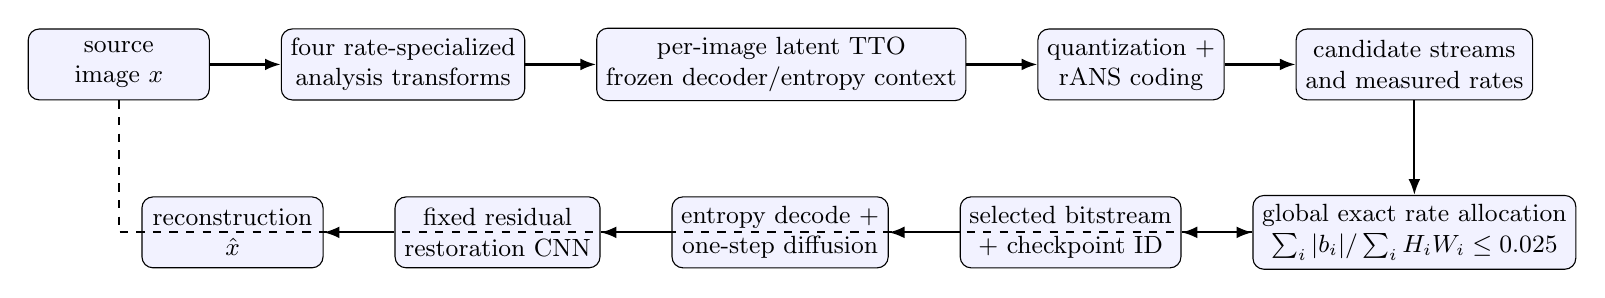
\begin{tikzpicture}[font=\small, node distance=7mm and 9mm,
 box/.style={draw,rounded corners,align=center,minimum height=9mm,minimum width=23mm,fill=blue!5},
 arr/.style={-{Latex[length=2mm]},thick}]
\node[box] (src) {source\\image $x$};
\node[box,right=of src] (multi) {four rate-specialized\\analysis transforms};
\node[box,right=of multi] (tto) {per-image latent TTO\\frozen decoder/entropy context};
\node[box,right=of tto] (rans) {quantization +\\rANS coding};
\node[box,right=of rans] (pool) {candidate streams\\and measured rates};
\node[box,below=12mm of pool] (knap) {global exact rate allocation\\$\sum_i |b_i|/\sum_i H_iW_i\leq0.025$};
\node[box,left=of knap] (stream) {selected bitstream\\+ checkpoint ID};
\node[box,left=of stream] (dec) {entropy decode +\\one-step diffusion};
\node[box,left=of dec] (enh) {fixed residual\\restoration CNN};
\node[box,left=of enh] (out) {reconstruction\\$\hat{x}$};
\draw[arr] (src)--(multi); \draw[arr] (multi)--(tto); \draw[arr] (tto)--(rans);
\draw[arr] (rans)--(pool); \draw[arr] (pool)--(knap); \draw[arr] (knap)--(stream);
\draw[arr] (stream)--(dec); \draw[arr] (dec)--(enh); \draw[arr] (enh)--(out);
\draw[arr,dashed] (src.south) |- (knap.west);
\end{tikzpicture}}
\caption{Final compression pipeline. Dashed flow denotes encoder-only access to the source for candidate evaluation and rate allocation; the submitted decoder receives only the selected bitstream and reconstructs without any source access.}
\label{fig:pipeline}
\end{figure}

\subsection{Backbone: AEIC-ME with a one-step diffusion prior}
\label{sec:backbone}
The base codec is the ME variant of AEIC~\cite{zhang2026aeic}, a one-step diffusion image codec whose analysis side maps RGB content into a compact quantized latent governed by a learned autoregressive entropy model, and whose synthesis side conditions an SD-Turbo one-step diffusion network~\cite{sauer2023sdturbo} on the decoded latent. SD-Turbo supplies a high-capacity natural-image prior while avoiding the sampling-step cost of the multi-step latent diffusion models it is distilled from~\cite{rombach2022ldm}. Our decoder bundle uses the trimmed FP16 SD-Turbo UNet and VAE together with the AdcSR half-decoder used by the AEIC implementation for the final pixel-space decode; large images are reconstructed using overlapping latent and VAE tiles, with overlap exceeding the effective local receptive boundary so that seams are not visible while peak activation memory stays bounded on a single consumer/cloud GPU.

\subsection{Rate-specialized checkpoint bank and bitstream signaling}
Zero-shot AEIC checkpoints are tuned for a broad rate ladder rather than for this challenge's exact 0.025 BPP AIGC operating point (\cref{tab:e1e3}). We fine-tuned four checkpoints starting from the public AEIC-ME initialization, varying the rate and reconstruction loss weights so that the four checkpoints cover complementary rate/perception regions rather than four points on an otherwise identical curve. Every checkpoint shares the same decoder entry point: the encoder writes one leading byte selecting the checkpoint, and the remainder is decoded by the shared practical entropy coder. This makes per-image model selection reproducible from the bitstream alone at negligible overhead. \Cref{tab:ckpts} documents the four checkpoints' training configuration; all four freeze the SD-Turbo/AdcSR diffusion decoder (\cref{sec:backbone}) and update only AEIC's analysis transform and entropy model.

\begin{table}[t]
\centering\scriptsize
\begin{tabular}{@{}lllcc@{}}
\toprule
Checkpoint & Init & Steps & Corpus & Target rate \\
\midrule
aigc8\_5000 & ft8 (zero-shot, $\lambda_8$) & 5k & train-800 + synth. & 0.020 BPP \\
r2\_18000 & aigc4\_5000 ($\lambda_4$) & 16k+ & real-800, 8$\times$ oversampled & 0.037 BPP \\
r3l4\_8000 & r2\_18000 & 8k & SD3.5+SDXL synth. & 0.037 BPP \\
r3l8\_8000 & aigc8\_5000 & 8k & SD3.5 synth. & 0.026 BPP \\
\bottomrule
\end{tabular}
\caption{Training configuration of the four shipped checkpoints. All four use AEIC's codec loss $\lambda_{\mathrm{rate}}R+\lambda_{2}\|x{-}\hat x\|_2^2+\lambda_{\mathrm{DISTS}}\mathcal{L}_{\mathrm{DISTS}}+\lambda_{\mathrm{CLIP}}\mathcal{L}_{\mathrm{CLIP}}+\lambda_{\mathrm{adv}}\mathcal{L}_{\mathrm{adv}}+\lambda_{\mathrm{LPIPS}}\mathcal{L}_{\mathrm{LPIPS}}$ ($\lambda_{\mathrm{adv}}{=}0$ for all four); only r2\_18000's $\lambda_{\mathrm{LPIPS}}{=}2.0,\lambda_{\mathrm{DISTS}}{=}1.5$ were separately logged, so exact retraining of the other three from this paper alone is not guaranteed; the shipped checkpoints, not this table, are the reproducibility artifact. Target rate is each checkpoint's natural operating point (\cref{tab:e1e3}), not an imposed constraint.}
\label{tab:ckpts}
\end{table}

\subsection{Encoder-side latent test-time optimization}
\label{sec:tto}
For the rf500 candidate (the only TTO-derived member of the 10-tag knapsack pool, \cref{sec:knapsack}), TTO refines the continuous pre-quantization latent $y$ with Adam (lr $10^{-3}$, no schedule) for 500 iterations (earlier development used 300; \cref{sec:ablation} reports that history), freezing all decoder weights and, within each refreeze interval (below), the entropy model's autoregressive conditioning. Quantization uses a straight-through estimator, $\hat y=\mathrm{STE\text{-}round}(y-\mu)+\mu$. Each iteration samples one random latent crop ($LY{=}16$, i.e.\ 512 source px; a text-box crop is sampled instead with probability 0.7 when available, weighting DISTS $3\times$ on that iteration), decodes it through the frozen one-step diffusion path (no restorer in this loop -- see below), and computes
\begin{equation}
 \mathcal{L}_{\mathrm{TTO}}=\lambda_2\|x-\hat{x}\|_2^2+40\,\mathcal{L}_{\mathrm{LPIPS}}+\lambda_D\mathcal{L}_{\mathrm{DISTS}}+\lambda_R R,
 \label{eq:tto}
\end{equation}
with $\lambda_2{=}1000$ (\texttt{mse\_w}), $\lambda_D{=}40$ (\texttt{dists\_w}, $\times3$ on text-biased iterations), $\lambda_R{=}20000$ (\texttt{rate\_w}), and the LPIPS coefficient fixed at 40; all are the unmodified defaults of our release, left untouched by any candidate-specific tuning. $R=\mathrm{ReLU}(\hat{r}-r_0)$ is a hinge penalty against the trajectory's own \emph{starting} rate $r_0$ (stop-gradient), so TTO is only penalized for exceeding where it began, not driven toward a target rate; $\hat r$ is the entropy model's differentiable rate \emph{estimate} (negative log-likelihood of $y$ under the frozen Gaussian conditional, in bits per pixel) -- a standard soft proxy, \emph{not} the true rANS bit count, since arithmetic coding is not differentiable. This estimate is used only to steer the trajectory; after every trajectory the final $y$ is re-quantized and passed through the actual, non-differentiable rANS entropy encoder, so every reported/scored/legal-budget bit count in this paper (\cref{tab:ablation,tab:results,tab:leaderboard}) is a measured file size, never the estimate. One TTO trajectory is run per (checkpoint, iteration-budget) candidate we chose to screen -- no random restarts or early stopping -- and the finished, fixed-iteration-count candidates are handed unmodified to the knapsack (\cref{sec:knapsack}), which is the only place selection happens. Text boxes are produced once, offline, by running the pretrained EasyOCR detector over each source image on the encoder side; they only bias TTO's crop sampling and are never transmitted or used by the decoder.

\paragraph{Conditioning refresh.} Because the autoregressive entropy context is derived from the latent being optimized, freezing it for the entire trajectory causes the context used to score candidate updates to grow stale as the latent moves. Periodically re-deriving the frozen context from the current latent every 75 iterations (\emph{refreeze}) was the single largest lever found during development: at matched 300-step budget it converted a marginal, sign-mixed effect (mean $-0.003$/img on a raw, uncapped 8-image screen) into a consistently positive one (6/8 images improved, one outlier at $-1.02$), and adding it to the legal-rate knapsack pool (v17$\to$v20, \cref{tab:ablation}) gave a confirmed +0.14 $S$ at matched legal rate. Extending trajectory depth from 300 to 500 steps under the same refreeze schedule (v20$\to$v21) added a further, dev-set-estimated +0.17 $S$, still not fully saturated at 500 steps per a shorter 800-step screen. Every component in \cref{tab:ablation}, including v20 and v21, was developed and frozen into the submitted codec before the July 20, 2026 Code Submission Phase deadline; only the post-deadline MBT2018-mean follow-up in \cref{sec:discussion} was conducted after the final test-phase submission and is explicitly excluded from it. TTO is strictly an encoder-side operation: the submitted decoder performs no optimization, gradient computation, or online adaptation of any kind.

\subsection{Global exact rate allocation}
\label{sec:knapsack}
Given candidate streams for image $i$ from checkpoint/refinement combination $j$, with challenge score $s_{ij}$ (computed against the source image, available to the encoder but not transmitted) and \emph{measured} coded length $r_{ij}$ bits, final per-image selection solves the multiple-choice knapsack
\begin{align}
 \max_{z_{ij}}\;&\sum_{i,j}s_{ij}z_{ij},\\
 \text{s.t. }&\sum_jz_{ij}=1\ \ \forall i,\quad
 \sum_{i,j}r_{ij}z_{ij}\leq0.025\sum_iH_iW_i,
\end{align}
with binary $z_{ij}$, solved to proven optimality with SciPy's \texttt{scipy.optimize.milp} (HiGHS branch-and-bound): one binary variable per (image, candidate), one equality row per image ($\sum_jz_{ij}=1$), one global inequality row on total bits, default presolve tolerance, 600\,s time limit (never approached; solve time is a few seconds for the $\sim\!1000$ variables in our 10-candidate$\times$100-image pool). Since \cref{eq:score} is linear in the four per-image metrics, the organizers' aggregate score equals $\frac{1}{|N|}\sum_{i,j}s_{ij}z_{ij}$ exactly, so maximizing this linear objective is provably equivalent to maximizing the organizers' true aggregate score, not an approximation to it. Two implementation details mattered: the rate constraint must use \emph{true pixel-weighted} bits-per-pixel ($\sum r_{ij}z_{ij}/\sum H_iW_i$), not a mean of per-image BPP values, since test images vary substantially in resolution; and $r_{ij}$ must be the actual on-disk file size (including the header byte), since fixed per-file overhead is non-negligible for small images at this bitrate. Both $s_{ij}$ and $r_{ij}$ are real measurements from reconstructed images and coded files, computed before the solver runs. Replacing an earlier greedy/Lagrangian remix (naive mean-BPP proxy) with this formulation was worth +0.0375 $S$ at fixed legal rate on its own (v17, \cref{tab:ablation}).

\subsection{Decoder-side residual restoration}
\label{sec:restorer}
The final stage is a fixed, eight-block residual CNN with dense local feature reuse per block (each block concatenates its input with intermediate features before a final $3\times3$ convolution), applied identically to every reconstruction regardless of which checkpoint produced it. The network is identity-initialized through a zero-initialized final convolution, predicts a bounded RGB residual, consumes no source pixels or side information, and therefore adds zero additional BPP. Its role is conservative correction of recurring color, edge, and local-texture error rather than unconstrained detail generation; on a separate 6-image subset (not the submitted TTO) we additionally routed TTO's gradient through this frozen restorer and found no improvement (mean $-0.036$ $S$, mixed signs, within noise), so this variant was rejected and the submitted TTO trajectory (\cref{sec:tto}) always optimizes against the raw, pre-restoration decode. See \cref{sec:ablation} for the restorer's independent, rate-orthogonal ablation.

\paragraph{Limitation.} The official metrics were computed from the organizer-scored reconstruction archive. The submitted bitstreams are independently decodable by the shipped decoder. For four images, encoder-side selection retained the raw reconstruction, whereas the standalone decoder applies restoration unconditionally; those four decoded outputs therefore differ from the archived PNGs.

\subsection{Implementation and reproducibility}
The submitted decoder bundle contains the trimmed FP16 SD-Turbo UNet/VAE, the AdcSR half-decoder, the four AEIC-ME checkpoints, the restoration weights, the practical entropy-coding extension, inference scripts, dependency notes, and a README, totalling approximately 4.76\,GB unpacked -- under the 5\,GB decoder-package limit. Because the decoder must be able to instantiate any of the four checkpoints depending on which byte it reads, all four codec networks (each including its own copy of the diffusion synthesis path) are resident on the GPU simultaneously during a decode run over a mixed-checkpoint bitstream directory; we found this leaves materially less headroom than a single-checkpoint decode, and a naive full-resolution application of the restoration network on top of this baseline memory footprint can exceed a 22--24\,GB GPU's budget on the largest ($>2048\times2048$) test images. Because the restoration network is a purely local, normalization-free convolutional stack, we apply it with overlapping-tile inference (tile size 512\,px, context padding 48\,px, comfortably larger than its $\approx$26-pixel receptive-field radius) so that peak activation memory is bounded independently of image resolution while producing output numerically identical to a single full-image forward pass. Reproduction requires Python 3.10, PyTorch 2.1.x with a CUDA 12.x-compatible runtime, CompressAI 1.2.8~\cite{begaint2020compressai}, Diffusers, xFormers, and the compiled rANS extension included by the build procedure.

\paragraph{Runtime.} The 8.5\,s/image figure in \cref{tab:results} is \emph{decoder-only} (standalone \texttt{decode.py}, one A10G); it excludes encoding. Of the 10 candidate tags/image (\cref{sec:knapsack}), only \emph{one} involves TTO: 4 raw checkpoint compressions (a few seconds/image total) plus their 4 zero-additional-bit enhancer variants, and one 500-step refreeze-75 TTO trajectory (\cref{sec:tto}) plus its enhanced copy (rf500/rf500\_enh share that single trajectory). TTO averaged 225.0\,s/image (99 images logged, 212.7--245.1\,s range) and dominates cost; encoding the 100-image submitted archive (100 TTO trajectories plus the cheap raw/enhancer passes) took approximately 6.5 A10G-hours, trivially shardable across images.

\section{Experiments}
\subsection{Training data}
The official benchmark, AIGC-IC-1000, contains 1000 images generated by 10 text-to-image models (100 images each) with prompts drawn from GenEval, DPG-Bench, and CVTG-2K (280 images each) and LongText-Bench (160 images), split 800/100/100 into train/validation/test; validation and test images preserve the original generator output resolution (mixed 1K/2K tiers) with no resize, crop, or padding. We used the 800 challenge-provided AIGC training images and additionally generated approximately 15{,}700 synthetic AIGC images from public prompt collections representing GenEval, DPG-Bench, CVTG-2K, and LongText-Bench styles, using publicly available SDXL, SD3.5-medium, PixArt-Sigma, and Sana models. The external corpus was used only for codec/domain fine-tuning and restoration training; challenge validation and test images were never used for gradient updates, checkpoint fitting, or decoder adaptation. \textbf{Extra training data was used and is disclosed here}, consistent with the challenge factsheet requirement. Training samples were randomly cropped and horizontally flipped; mixed image sources and multiple codec-rate reconstructions were sampled during restoration training so the restorer did not specialize to a single rate point.

\paragraph{Provenance.} We generated our synthetic corpus ourselves, by sampling from the public GenEval, DPG-Bench, CVTG-2K, and LongText-Bench prompt \emph{collections} at their default public releases, using SDXL, SD3.5-medium, PixArt-Sigma, and Sana at their default public checkpoint revisions. This means our corpus and the organizers' training split draw from the same named public prompt sources, not that we reused the organizers' specific prompt selections or generated images: we never had access to the organizers' exact prompt lists, generation seeds, or output images for any split, including training. The organizers' validation and test images come from a separate, non-public generation the organizers alone control, and no validation or test image was ever used for a gradient update, checkpoint selection, or decoder adaptation at any stage of the pipeline.

\subsection{Training protocol}
\label{sec:training-protocol}
Codec fine-tuning started from the public AEIC-ME checkpoint and retained the public SD-Turbo/AdcSR initialization; the four rate-specialized checkpoints were produced by varying rate and reconstruction loss weights rather than by training distinct architectures. Training used Adam/AdamW-family optimization with cosine learning-rate decay; the initial learning rate was approximately $2\times10^{-4}$ for the restoration module. Restoration batches used random patches up to $384\times384$ and batch size 8, with gradients clipped to unit norm. The restoration loss combined L1 pixel error, LPIPS, DISTS, and an edge-aware DISTS term; an adversarial loss was evaluated during development but disabled in the final model because it improved apparent sharpness at the cost of distortion and text fidelity. Checkpoint selection used actual reconstructed validation images and real, measured stream lengths, jointly considering PSNR, MS-SSIM, LPIPS, DISTS, BPP, and standalone-decoder reproducibility.

\subsection{Evaluation protocol}
\label{sec:eval}
The organizers' score combines all four metrics as
\begin{equation}
S=\mathrm{PSNR}+10\,\mathrm{MS\mbox{-}SSIM}+40(1-\mathrm{LPIPS})+40(1-\mathrm{DISTS}),
\label{eq:score}
\end{equation}
equivalently $S = \mathrm{PSNR} + 10\,\mathrm{MS\mbox{-}SSIM} - 40\,\mathrm{LPIPS} - 40\,\mathrm{DISTS} + 80$, i.e. $S$ is exactly the sum of the four raw metrics as written in the organizers' rules. We verified our local evaluation reproduces the organizers' \emph{displayed} leaderboard number digit-for-digit across every submission for which both were available before the final test phase, and found that displayed number to equal $B \triangleq S - 80$ in every case (e.g.\ our own official entry: $S=111.527739$, displayed $B=31.527739$; \cref{tab:results}). \textbf{Scale convention for this paper:} development tables (\cref{tab:e1e3,tab:ablation}) report the unshifted $S$, matching our development log; official leaderboard results (\cref{tab:results,tab:leaderboard}) and any number explicitly marked ``board''/$B$ report $B=S-80$, the organizers' displayed scale. Every table and in-text number states or is adjacent to its scale; where both appear together (e.g.\ \cref{sec:discussion}), each value is individually labeled. The organizers determine the final test-phase ranking from two perspectives: (i) this objective score, and (ii) a subjective assessment of content consistency and perceptual quality from human annotations; the awards are correspondingly split into two non-overlapping objective-performance awards and three perceptual-performance awards. \Cref{tab:leaderboard} reports the objective-score ranking, which is the only leaderboard released to participants at the time of writing; our system was optimized solely against \cref{eq:score} and was not tuned against any human-preference signal.

\begin{table}[t]
\centering\footnotesize
\begin{tabular}{@{}lccc@{}}
\toprule
Checkpoint & Nominal rate & Score & BPP \\
\midrule
ft8 (zero-shot) & low & 106.19 & 0.017 \\
ft4 (zero-shot) & mid & 109.21 & 0.0239 \\
ft2 (zero-shot) & high & 111.28 & 0.031 \\
Knapsack mix (v1) & -- & 109.55 & 0.0250 \\
\bottomrule
\end{tabular}
\caption{Zero-shot AEIC-ME rate ladder on the challenge validation set, before any AIGC fine-tuning, TTO, or restoration ($S$ scale, i.e. leaderboard scale $+80$; see \cref{sec:eval}). A single checkpoint at the legal rate already trails a per-image mix of unrelated rate points, motivating the checkpoint-bank design used throughout the rest of the system. Under the same early (mean-BPP-constrained, later superseded) solver, adding three fine-tuned checkpoints to this pool raised the mix from 109.55 to 109.89 (+0.34) -- a same-methodology signal fine-tuning was worth adding, not comparable to \cref{tab:ablation}'s later rows.}
\label{tab:e1e3}
\end{table}

\subsection{Main results}
\Cref{tab:results} reports our official final-test-phase metrics as recalculated and announced by the organizers on August 4, 2026. \Cref{tab:leaderboard} reproduces the organizer-announced final ranking for all ten verified entries. We rank 5th; the top four entries all report substantially higher PSNR (28.6--29.8\,dB against our 27.0\,dB) at comparable or tighter BPP, while our DISTS (0.038970) is second-lowest of all ten entries -- only prophet1 (0.038851, ranked 6th) is lower -- and the lowest among every entry ranked above us.

\begin{table}[t]
\centering\small
\begin{tabular}{@{}lc@{}}
\toprule
Quantity & Final test entry \\
\midrule
Official score ($B{=}S{-}80$) & 31.527739 \\
PSNR & 27.022356 dB \\
MS-SSIM & 0.917594 \\
LPIPS & 0.077794 \\
DISTS & 0.038970 \\
Average BPP & 0.024946 \\
Reported runtime & 8.5 s/image \\
Execution device & GPU \\
\bottomrule
\end{tabular}
\caption{Official organizer-recalculated final-test metrics for the submitted entry.}
\label{tab:results}
\end{table}

\begin{table}[t]
\centering\scriptsize
\resizebox{\textwidth}{!}{%
\begin{tabular}{@{}clcccccc@{}}
\toprule
Rank & Team & Score & BPP & PSNR & MS-SSIM & LPIPS & DISTS \\
\midrule
1 & Ashes & 34.004381 & 0.025000 & 29.820286 & 0.930888 & 0.076335 & 0.051785 \\
2 & rrrrty & 33.557593 & 0.024987 & 28.926965 & 0.934522 & 0.071049 & 0.046815 \\
3 & NeFIC++ & 33.271115 & 0.024153 & 28.601395 & 0.932167 & 0.071724 & 0.044575 \\
4 & Freedom & 32.849392 & 0.025000 & 28.779010 & 0.933339 & 0.077461 & 0.054115 \\
\rowcolor{blue!8}
5 & \textbf{Ours} & \textbf{31.527739} & \textbf{0.024946} & \textbf{27.022356} & \textbf{0.917594} & \textbf{0.077794} & \textbf{0.038970} \\
6 & prophet1 & 30.349026 & 0.024962 & 26.303701 & 0.908165 & 0.087057 & 0.038851 \\
7 & qrchen & 30.183789 & 0.024948 & 27.740318 & 0.917277 & 0.109328 & 0.058905 \\
8 & Team-Team & 29.318431 & 0.023415 & 26.729861 & 0.915676 & 0.104364 & 0.059841 \\
9 & rohit\_choudhary & 28.221412 & 0.024785 & 27.014252 & 0.904016 & 0.126391 & 0.069434 \\
10 & aigilic & 27.979867 & 0.021782 & 26.129605 & 0.902043 & 0.114655 & 0.064599 \\
\bottomrule
\end{tabular}}
\caption{Official final test-phase leaderboard, organizer-recalculated and announced August 4, 2026, at full precision. Our DISTS (0.038970) is second-lowest overall (only prophet1's 0.038851 is lower) and lowest among every entry ranked above us; our LPIPS is not a leadership position. PSNR trails the top four by 1.6--2.8\,dB (\cref{sec:discussion}).}
\label{tab:leaderboard}
\end{table}

\subsection{Qualitative results}
\Cref{fig:qual} shows two test images decoded from the actual submitted bitstream: a text-heavy retail-poster scene (000009, 0.0189 BPP) and a lower-frequency interior scene (000071, 0.0129 BPP); both are individually \emph{below} the 0.025 average -- the knapsack (\cref{sec:knapsack}) spends more elsewhere and these are not the most rate-expensive examples in the set. Rendered typography (``GEAR UP'', ``BEST DEALS'', ``LIMITED EDITION'', the brand wordmark) and fine repeated structure (the shoe rack, folded-garment texture) remain legible and structurally faithful to the source, illustrating the leaderboard-level DISTS strength reported in \cref{tab:leaderboard}. We hand-selected these two images to show a text-heavy and a low-frequency example side by side; the quantitative claims in this paper rest on the full-set numbers in \cref{tab:leaderboard,tab:ablation}, not on this figure.

\begin{figure}[t]
\centering
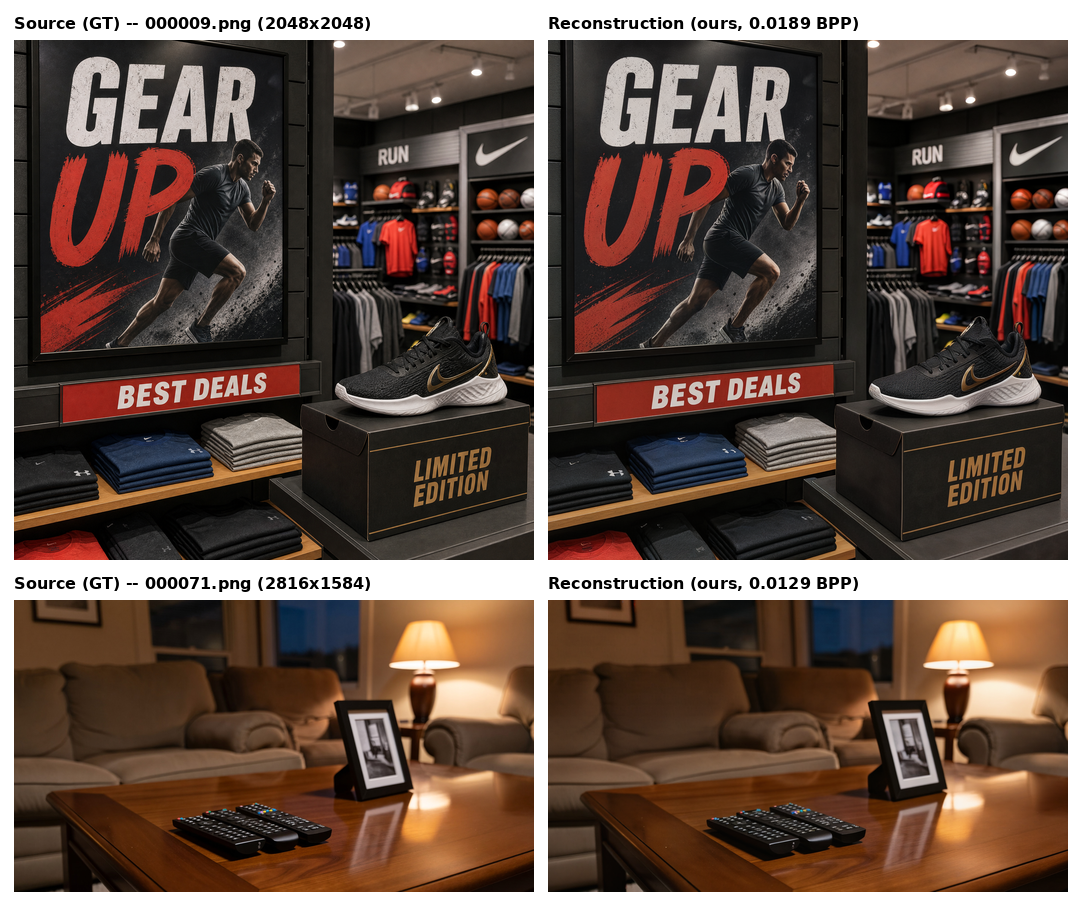
\includegraphics[width=\textwidth]{qualitative.png}
\caption{Source (ground truth) vs.\ our reconstruction, decoded from the actual submitted bitstream using the shipped decoder. Top: 000009.png, 0.0189 BPP. Bottom: 000071.png, 0.0129 BPP. Hand-selected for content type (text-heavy vs.\ low-frequency), not randomly sampled; see \cref{sec:ablation} for the quantitative, full-set evidence.}
\label{fig:qual}
\end{figure}

\subsection{Submission progression and development history}
\label{sec:ablation}
\Cref{tab:ablation} traces the submitted system's development, drawn from a development log of 77 tracked experiments spanning July 5--31, 2026. \textbf{Every row is a full knapsack-mixed submission candidate at the true legal weighted-bpp rate ($\leq0.025$), not a raw per-candidate number.} The first two rows (v1$\to$v17) jointly add fine-tuning, 300-step TTO, and the exact MILP solver and should be read as a combined-methodology jump, not an isolated ablation; only the later transitions (v17$\to$v20 adds conditioning refresh, v20$\to$v21 adds 500-step TTO) add exactly one component to the candidate pool the knapsack (\cref{sec:knapsack}) may choose from, so only those two deltas are directly attributable to a single addition at matched legal rate. The +0.0375 exact-MILP-over-greedy delta reported in \cref{sec:knapsack} is a separately matched comparison (same candidate pool, only the solver changed) and is not the v1$\to$v17 delta. Rows marked \emph{confirmed} were independently scored by the organizers' own leaderboard; rows marked \emph{dev-set est.} were solved locally on the validation set only and not separately submitted. All scores are on the $S$ scale (\cref{sec:eval}).

\begin{table}[t]
\centering\scriptsize
\begin{tabular}{@{}lccl@{}}
\toprule
Candidate pool (cumulative) & $S$ & BPP & Status \\
\midrule
Zero-shot checkpoints only (v1) & 109.94 & 0.0250 & confirmed \\
+ fine-tuning, 300-step TTO, exact MILP (v17) & 111.53 & 0.0250 & confirmed \\
\quad + conditioning refresh (v20) & 111.66 & 0.0250 & confirmed \\
\quad\quad + 500-step TTO (v21) & 111.83 & 0.0250 & dev-set est. \\
Official organizer-scored archive (test) & 111.53 & 0.0249 & confirmed (test) \\
\bottomrule
\end{tabular}
\caption{Legal-rate ($\leq0.025$ BPP) knapsack-mixed submission progression on the validation set, except the last row (official test set). The dev-set v21 estimate (111.83) does not match the confirmed official test score (111.53): validation-set gains from the deepest TTO schedule did not fully transfer to the held-out test images.}
\label{tab:ablation}
\end{table}

\paragraph{Restoration network.} Because the fixed residual restorer (\cref{sec:restorer}) is applied post-decode with zero additional bits, its effect is rate-orthogonal and does not require a matched-rate comparison: applying it to reconstructions from every candidate checkpoint type gave a uniform +0.22 $S$ average gain (range +0.19 to +0.25 across candidate types, 100-image validation set), and extending its training from 8k to 18k steps on the same fixed L1+LPIPS+DISTS objective (no adversarial loss, no architecture change) raised this further to +0.27, confirming the gain came from training duration rather than loss-function or capacity changes -- a 16-block (2$\times$-capacity) variant tested at matched convergence scored slightly \emph{worse} (111.25 vs.\ 111.27 $S$ on a fixed candidate set), closing out the architecture search.

\paragraph{Candidate-level screening (uncapped rate).} These, measured on raw reconstructions or small subsets, decided what to \emph{add} to the legal-rate pool in \cref{tab:ablation}, not standalone legal-rate claims: wider TTO crop context (\texttt{crop\_ly} 16$\to$24) was net-negative once re-mixed through the knapsack; MSE weight 1000$\to$300$\to$0 monotonically hurt score (29.88$\to$29.82$\to$29.79 $S{-}80$), so it stabilizes the search rather than only trading off perceptual terms; DISTS surrogate weight 40$\to$80$\to$120 didn't improve whole-image DISTS and damaged LPIPS/PSNR; multi-seed TTO was seed-insensitive; checkpoint weight-souping underperformed both parents; cross-family fusion with OSCAR~\cite{guo2025oscar}/OneDC~\cite{xue2025onedc} was non-competitive (\cref{sec:related}).

\section{Discussion: the PSNR gap}
\label{sec:discussion}
After the final test-phase result was announced, we investigated whether the PSNR gap to the top four entries (1.6--2.8\,dB) could be closed by remixing existing candidates or by re-weighting the TTO objective. Two experiments give two different strengths of evidence and we report them separately rather than pooling them.

\paragraph{Full-validation-set evidence (robust, $n{=}100$).} Re-solving the existing ten-candidate pool over all 100 validation images with PSNR weighted 1$\times$, 2$\times$, and 4$\times$ relative to the other three metrics raised the achievable PSNR at the legal bitrate to only 27.08\,dB -- a 0.06\,dB improvement -- while lowering the combined score from $B{=}31.53$ to $31.48$, because every additional PSNR-weighted candidate choice cost more in LPIPS/DISTS than it gained in PSNR under \cref{eq:score}. This is a full-validation-set, exact-MILP result and we consider it solid: \emph{given the candidates already in our pool}, re-weighting the selection criterion cannot raise PSNR by more than about 0.06\,dB at this rate.

\paragraph{Small-sample screen (preliminary, $n{=}4$).} We separately added an explicit, differentiable PSNR term ($10\log_{10}(1/\mathrm{MSE})$) directly into the TTO objective (\cref{eq:tto}) and re-ran the 500-step/refreeze-75 schedule on four representative test images: mean PSNR was 26.05\,dB against the existing rf500-enh candidate's 26.16\,dB on the same four images, with per-image deltas of $+0.057$, $-0.562$, $+0.121$, $-0.060$\,dB and simultaneous regression of the perceptual metrics. With $n{=}4$ and no dispersion estimate, this cannot by itself rule out that a different learning rate, weight schedule, or longer trajectory would recover the PSNR term's intended effect; we report it as a preliminary negative signal, not proof.

\paragraph{Interpretation.} Together with the full-pool result above and our observation that generic distortion-oriented codecs improved PSNR on selected images at the cost of substantially worse LPIPS/DISTS (why they were not used), we consider it \emph{likely} rather than proven that the residual PSNR gap reflects the one-step diffusion synthesis path itself, not a loss-weighting artifact correctable within our pool; closing it would plausibly need a higher-fidelity training objective or a smaller generative degrees-of-freedom budget. Under \cref{eq:score}, our confirmed strength is DISTS (second-best overall, best among the top five), not PSNR or LPIPS (\cref{tab:leaderboard}).

\paragraph{Post-deadline follow-up.} No changes are permitted after the Code Submission Phase (2026-07-20); this ran afterward on the validation set and is \emph{not} part of the submitted entry. Testing whether a different, fidelity-trained family could close the PSNR gap (\cref{sec:discussion}), we added a reduced-resolution MBT2018-mean path (12-block decoder, 800 real reconstructions): 27.30\,dB PSNR @ 0.0257\,BPP, but LPIPS/DISTS both worse than AEIC's. As a knapsack family it was selected for only 6/100 images (+0.055 $S$) -- it raises the PSNR ceiling, but its perceptual cost outweighs the gain almost everywhere. Closing the gap needs a family both higher-fidelity \emph{and} perceptually competitive, not a larger pool alone.

\section{Ensembles and Multi-Model Strategies}
The submitted method is a multi-model \emph{rate} ensemble, not an output-image ensemble: one stream and checkpoint identifier are selected per image, with no pixel averaging, oracle information, or multiple decoder outputs. All four checkpoints and the selection signaling are part of the submitted codec; the global allocator (\cref{sec:knapsack}) is encoder-only, with no source-dependent fallback logic in the shipped decoder. Every submitted bitstream is independently decodable by the shipped decoder.

\section{Conclusion}
We presented our submission: four fine-tuned AEIC-ME checkpoints, encoder-side latent TTO with entropy-conditioning refresh, exact knapsack rate allocation over real coded bitstream sizes, and a fixed zero-rate restoration network, reaching rank 5 (score 31.527739, second-best DISTS) while trailing the top four on PSNR. Given the split award tracks (\cref{sec:eval}), the perceptual track fits better here. This gap likely reflects the diffusion backbone's fidelity/perception trade-off, not a tunable loss weight (\cref{sec:discussion}); fine-tuning or replacing the base codec's fidelity objective is the most promising path forward.

\paragraph{Compliance statement.} The described codec/checkpoints are those submitted for the Code Submission Phase; the test archive used that codec, with no decoder update or fine-tuning afterward, and TTO does not modify decoder weights (pretrained components: \cref{sec:backbone}; extra data: Sec.~4.1).

\bibliographystyle{splncs04}
\bibliography{egbib}
\end{document}
